\usetikzlibrary{arrows}
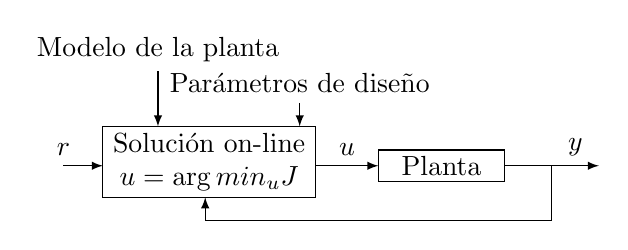
\begin{tikzpicture}
\draw  (1.8,4) rectangle (3.4,3.6) node[midway, align=center] {Planta};





\draw [-latex](3.4,3.8) -- (4.6,3.8) node[above, near end] {$y$};




\draw [-latex](4,3.8) -- (4,3.1) -- (-0.4,3.1)-- (-0.4,3.4);


\draw [-latex](-2.2,3.8) node[above] {$r$} -- (-1.7,3.8);
\draw  (-1.7,4.3) rectangle (1,3.4) node[midway, align=center] {Solución on-line\\$u=\arg min_u J$};
\draw [-latex](1,3.8) -- (1.8,3.8) node[above, midway]{$u$};
\draw [-latex](-1,5) node[above]{Modelo de la planta} -- (-1,4.3);
\draw [-latex](0.8,4.6) node[above]{Parámetros de diseño}  -- (0.8,4.3);
\end{tikzpicture}